\documentclass{beamer}
\usetheme{Antibes}
\usepackage{subcaption}
\usepackage{amsmath, amsfonts, amssymb}
\usepackage{stmaryrd}
\usepackage{physics}
\setbeamertemplate{footline}[frame number]
\setbeamersize{text margin left=3mm} 

\AtBeginSection[]{
  \begin{frame}
  \vfill
  \centering
  \begin{beamercolorbox}[sep=8pt,center,shadow=true,rounded=true]{title}
    \usebeamerfont{title}\insertsectionhead\par%
  \end{beamercolorbox}
  \vfill
  \end{frame}
}

\DeclareMathOperator*{\argmin}{arg\,min}

\title{Diffusion Models: A Comprehensive Survey of Methods and
Applications, Part 1}
\subtitle{By Ling Yang, Zhilong Zhang, Yang Song, Shenda Hong, Runsheng Xu, Yue Zhao, Wentao Zhang, Bin Cui, Ming-Hsuan Yang}
\author{Presented by: Evgenii Samutichev}

\begin{document}

\maketitle

\begin{frame}{Outline}
    \small 
    \tableofcontents
\end{frame}

\section{Introduction (Chapter 1)}
\begin{frame}{Introduction (Chapter 1)}
\begin{itemize}
  \item New state-of-the-art family of deep generative models, which beat GANs on several tasks, including image synthesis (e.g. Stable Diffusion, DALL-E)
  \item The body of research on diffusion models has grown significantly, many interesting approaches and mathematics.
  \item \textbf{Key idea}: progressively perturbing data with intensifying random noise, while learning how to remove noise to generate new data samples.
\end{itemize}
\begin{figure}[h!]
  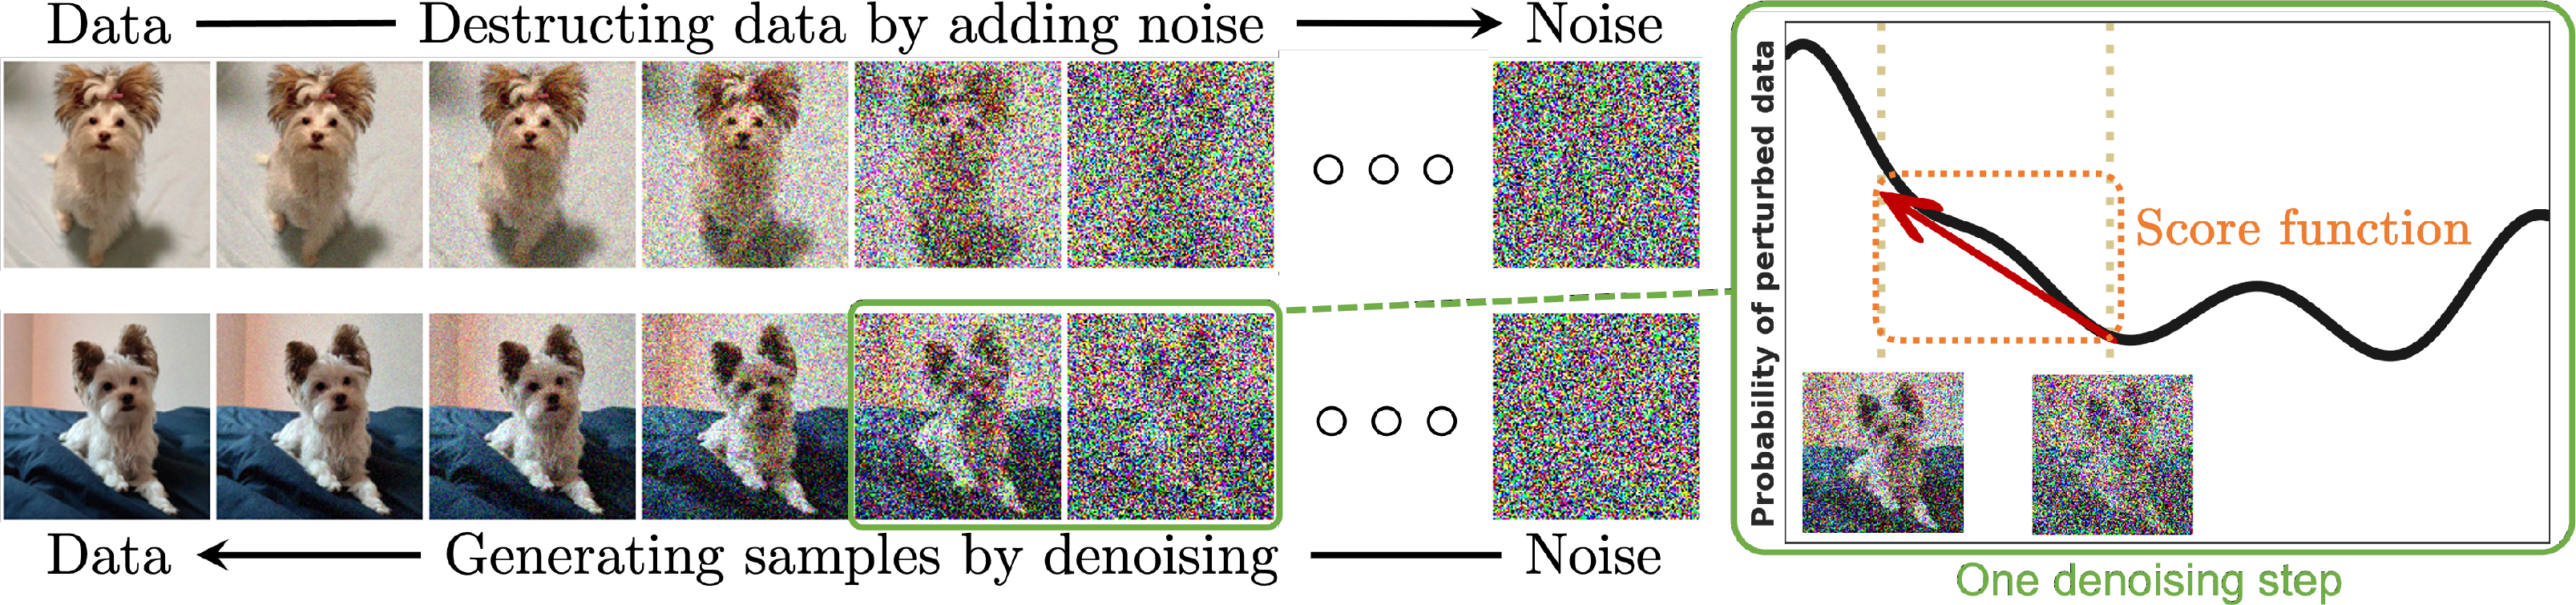
\includegraphics[width=0.9\textwidth]{diffusion.png}
  \centering 
\end{figure}
\end{frame}

\section{Three predominant mathematical formulations (Chapter 2)}
\subsection{Denoising diffusion probabilistic models (DDPMs)}
\begin{frame}{DDPM key ideas}
\begin{itemize}
  \item We first consider \textbf{Denoising diffusion probabilistic models (DDPMs)} formulation. 
  \item Two Markov chains: \textbf{forward} that introduces noise, \textbf{reverse} that converts noise back to data.
  \item Forward is typically hand-designed, reverse has to be learned 
  \item Starting from an unknown data distribution $\mathbf{x}_0 \sim q(\mathbf{x}_0)$, forward process $\mathbf{x}_1, ..., \mathbf{x}_T$ with transition kernel $q(\mathbf{x}_{t} \mid \mathbf{x}_{t-1})$. 
  \item Starting from some known noise distribution $\mathbf{x}_T \sim p(\mathbf{x}_T)$, reverse process with transition kernel $p_\theta(\mathbf{x}_{t-1} \mid \mathbf{x}_t)$ parametrized by deep neural networks, should generate $\mathbf{x}_{T-1}, ..., \mathbf{x}_0$.
\end{itemize}
\end{frame} 

\subsubsection{Forward process}
\begin{frame}{Forward process}
\begin{itemize}
  \item Joint distribution (chain rule of probability + Markov property)
  \begin{align}
    q(\mathbf{x}_1, ..., \mathbf{x}_T \mid \mathbf{x}_0) = \prod_{t=1}^{T}{q(\mathbf{x}_t \mid \mathbf{x}_{t-1}, ..., \mathbf{x}_0)} = \prod_{t=1}^{T}{q(\mathbf{x}_t \mid \mathbf{x}_{t-1})}\label{eq:marginal-q}
  \end{align}
  \item The most common choice is Gaussian 
  \begin{align}
    q(\mathbf{x}_{t} \mid \mathbf{x}_{t-1}) = \mathcal{N}(\mathbf{x}_t ; \sqrt{1-\beta_t}\mathbf{x}_{t-1},\beta_t \mathbf{I}), \quad \beta_t \in (0, 1)
  \end{align}
  \item \textbf{Sohl-Dickstein formula}
  \begin{align}
    q(\mathbf{x}_{t} \mid \mathbf{x}_{0}) = \mathcal{N}(\mathbf{x}_{t}; \sqrt{ \overline{\alpha}_{t} }\mathbf{x}_{0} , (1-\overline{\alpha}_{t} )\mathbf{I})
  \end{align}
  where $\alpha_{t} = 1 -\beta_{t}, \quad \overline{\alpha}_{t}=\prod_{s=0}^{t}{\alpha_{s}}$
  \item Then with the right choice of $\beta_t \in (0, 1)$, we have $q(\mathbf{x}_t \mid \mathbf{x}_0) \to \mathcal{N}(\mathbf{0}, \mathbf{I})$ as $t \to \infty$
\end{itemize}
\end{frame}

\begin{frame}{Sohl-Dickstein formula, a sketch of the proof (1 / 2)}
\begin{itemize}
  \item For two independent Gaussian kernels of the form $\mathcal{N}(\mathbf{x};\mu_{\mathbf{x}}, \beta_{\mathbf{x}}\mathbf{I})$ and $\mathcal{N}(\mathbf{y};\mu_{\mathbf{y}}, \beta_{\mathbf{y}} \mathbf{I})$, their product is another Gaussian kernel but for $\begin{bmatrix}\mathbf{x}\\ \mathbf{y}\end{bmatrix}$ with mean $\begin{bmatrix}\mu_{\mathbf{x}} \\ \mathbf{\mu}_{\mathbf{y}}\end{bmatrix}$ and covariance matrix $\begin{bmatrix}\beta_{\mathbf{x}}\mathbf{I} & 0 \\ 0 & \beta_{\mathbf{y}}\mathbf{I}\end{bmatrix}$. 
\end{itemize}
\begin{align*}
  q(\mathbf{x}_{1},\dots,\mathbf{x}_{T} \mid \mathbf{x}_{0})=\mathcal{N}\left(\mathbf{x}_{1},\dots,\mathbf{x}_{T};\begin{bmatrix}
\sqrt{\alpha_{1}}\mathbf{x}_{0} \\
\dots \\
\sqrt{\alpha_{T}}\mathbf{x}_{T-1}
\end{bmatrix}, \begin{bmatrix}
\beta_{1}\mathbf{I} & \cdots & 0 \\
0 & \cdots & 0 \\ 
0 & \cdots & \beta_{T}\mathbf{I}
\end{bmatrix}\right)
\end{align*}
\begin{itemize}
  \item Focusing only on $\mathbf{x}_1$ under the exponent
\end{itemize}
$$
 -\frac{1}{2\beta_{1}}(\mathbf{x}_{1}-\sqrt{ \alpha_{1} }\mathbf{x}_{0})^T(\mathbf{x}_{1}-\sqrt{ \alpha_{1} }\mathbf{x}_{0}) -\frac{1}{2\beta_{2}}(\mathbf{x}_{2}-\sqrt{ \alpha_{2} }\mathbf{x}_{1})^T(\mathbf{x}_{2}-\sqrt{ \alpha_{2} }\mathbf{x}_{1})
$$
\end{frame}

\begin{frame}{Sohl-Dickstein formula, a sketch of the proof (2 / 2)}
  \begin{itemize}
    \item Changing the variable $\mathbf{x}_{1} \to \frac{1}{\sqrt{ \alpha_{2} }} (\mathbf{x}_{2} - \mathbf{x}_{1})$, we get 
    $$
-\frac{1}{2\beta_{2}}\mathbf{x}_{1}^T \mathbf{x}_{1} - \frac{1}{2\beta_{1}\alpha_{2}}(\mathbf{x}_{1} -(\mathbf{x}_{2} - \sqrt{ \alpha_{1}\alpha_{2} }\mathbf{x}_{0}))^T (\mathbf{x}_{1} -(\mathbf{x}_{2} - \sqrt{ \alpha_{1}\alpha_{2} }\mathbf{x}_{0}))
$$
\item Then, use the formula 
\end{itemize}
\begin{align}
  \int_{\mathbf{R}^n}{\mathcal{N}(\mathbf{x}; \mathbf{0}, \Gamma)\mathcal{N}(\mathbf{x}; \mu, \Sigma) \dd \mathbf{x}} = \frac{\exp\left(-\frac{1}{2}\mu^T (\Gamma (\Sigma^{-1} + \Gamma^{-1})\Sigma)^{-1}\mu \right)}{\sqrt{(2\pi)^n |\Sigma||\Gamma||\Sigma^{-1} + \Gamma^{-1}|}}
\end{align}
\begin{itemize}
  \item to get under the exponent 
  \begin{align*}
    -\frac{1}{2(1-\alpha_{1}\alpha_{2})}(\mathbf{x}_{2} - \sqrt{ \alpha_{1}\alpha_{2} }\mathbf{x}_{0})^T (\mathbf{x}_{2} - \sqrt{ \alpha_{1}\alpha_{2} }\mathbf{x}_{0})
  \end{align*}
\end{itemize}
\end{frame}

\subsubsection{Reverse process}
\begin{frame}{Reverse process}
\begin{itemize}
  \item Learnable transition kernel, also Gaussian 
  \begin{align}
    p_\theta (\mathbf{x}_{t-1}\mid \mathbf{x}_t) = \mathcal{N}(\mathbf{x}_{t-1}; \mu_\theta (\mathbf{x}_t, t), \Sigma_\theta (\mathbf{x}_t, t))
  \end{align}
  with $\mu_\theta (\mathbf{x}_t, t), \Sigma_\theta (\mathbf{x}_t, t)$ represented by DNNs. 
  \item Joint distribution 
  \begin{align}
    p_\theta(\mathbf{x}_0, ..., \mathbf{x}_T) = p(\mathbf{x}_T) \prod_{t=1}^{T}{p_\theta(\mathbf{x}_{t-1} \mid \mathbf{x}_t)} \label{eq:marginal-p}
  \end{align}
\end{itemize}
\end{frame}

\subsubsection{Training DDPM with VLB loss}
\begin{frame}{Training DDPM with VLB loss}
\begin{itemize}
  \item We want to match the reverse process with the forward process in distribution, thus we start with KL-divergence as a loss 
  \begin{align*}
    \text{KL}(q(\mathbf{x}_0, ..., \mathbf{x}_T) \ || \ p_\theta(\mathbf{x}_0, ..., \mathbf{x}_T)) = -\mathbb{E}_{q(\mathbf{x}_0, ..., \mathbf{x}_T)}\left[\log \frac{p(\mathbf{x}_0, ..., \mathbf{x}_T)}{q(\mathbf{x}_0, ..., \mathbf{x}_T)}\right].
  \end{align*}
  \item Can be simplified to get the \textbf{Variational Lower Bound (VLB)} of the log-likelihood of the data $\mathbf{x}_0$
  \begin{align*}
    \text{KL}(q(\mathbf{x}_0, &..., \mathbf{x}_T) \ || \ p_\theta(\mathbf{x}_0, ..., \mathbf{x}_T)) = \\
    &= -\underbrace{\mathbb{E}_{q(\mathbf{x}_0, ..., \mathbf{x}_T)}\left[\log p(\mathbf{x}_T) + \sum_{t=1}^{T}{\log \frac{p_\theta(\mathbf{x}_{t-1} \mid \mathbf{x}_t)}{q(\mathbf{x}_t \mid \mathbf{x}_{t-1})}}\right]}_{L_{\text{VLB}(\mathbf{x}_0)}} + \text{const}
  \end{align*}
\end{itemize}
\end{frame}

\begin{frame}{More on VLB}
\begin{itemize}
  \item To better understand where VLB comes from, we first fix $\mathbf{x}_0$ and write by Jensen's inequality 
\begin{align}
-\log p_\theta(\mathbf{x}_0) \leq \mathbb{E}_{q(\mathbf{x}_1,...,\mathbf{x}_T  | \mathbf{x}_0)}\left[-\log \frac{p_\theta(\mathbf{x}_0, \mathbf{x}_1, ..., \mathbf{x}_T)}{q(\mathbf{x}_1,...,\mathbf{x}_T  | \mathbf{x}_0)}\right]
\end{align}
\item Then, we take expectation w.r.t. $\mathbf{x}_0 \sim q(\mathbf{x}_0)$ of both sides, and multiply by $-1$ resulting in 
\begin{align*}
\log p_\theta(\mathbf{x}_0) \geq  \mathbb{E}_{q(\mathbf{x}_0, \mathbf{x}_1,...,\mathbf{x}_T)}\left[\log \frac{p_\theta(\mathbf{x}_0, \mathbf{x}_1, ..., \mathbf{x}_T)}{q(\mathbf{x}_1,...,\mathbf{x}_T \mid \mathbf{x}_0)}\right] = L_{\text{VLB}(\mathbf{x}_0)}
\end{align*}
\item We can then use expressions \eqref{eq:marginal-q} and \eqref{eq:marginal-p} to get that connection with KL-divergence (maximizing one minimizes the other)
\end{itemize}
\end{frame}

\subsection{Score-based Generative Models (SGMs)}
\begin{frame}{SGM key ideas}
\begin{itemize}
  \item Next, consider \textbf{Score-based Generative Models (SGMs)} formulation. 
  \item Perturb data with a sequence of intensifying Gaussian noise and jointly estimate the score functions for all noisy data distributions by training a deep neural network model conditioned on noise levels (called a noiseconditional score network, NCSN).
  \item Given a PDF $p(\mathbf{x})$, the \textbf{Stein score function} is $\nabla_\mathbf{x} \log p(\mathbf{x})$.
  \item Consider a sequence of noise levels $0 < \sigma_1 < \sigma_2 < ... < \sigma_t < ... < \sigma_T$ and let $q(\mathbf{x}_t \mid \mathbf{x}_{0}) = \mathcal{N}(\mathbf{x}_t ; \mathbf{x}_0, \sigma_t^2 \mathbf{I})$, then $q(\mathbf{x}_t) = \int q(\mathbf{x}_t \mid \mathbf{x}_{0}) q(\mathbf{x}_0) \dd \mathbf{x}_0$.
  \item Want to estimate scores $\mathbf{s}_\theta (\mathbf{x}, t) = \nabla_{\mathbf{x}_t}\log q(\mathbf{x}_t)$ with DNN to then use as directions in the sampling algorithm based of Langevin dynamics.
\end{itemize}
\end{frame}

\subsubsection{Training SGM with denoising score matching}
\begin{frame}{Training SGM with denoising score matching (1 / 2)}
  \begin{itemize}
    \item \textit{Ho et al. (2020)} paper introduces the following loss function with weights $\lambda(t)$ for DDPM
    \begin{align}
      \mathbb{E}_{t \sim \mathcal{U}(\{1,...,T\}), \mathbf{x}_0 \sim q(\mathbf{x}_0), \boldsymbol{\epsilon}\sim \mathcal{N}(\mathbf{0}, \mathbf{I})}\left[\lambda(t) \norm{\boldsymbol{\epsilon}-\boldsymbol{\epsilon}_\theta(\mathbf{x}_t, t)}^2\right]
    \end{align}
    where $\boldsymbol{\epsilon}_\theta(\mathbf{x}_t, t)$ predicts added noise and we compute $\mathbf{x}_t$ based on Sohl-Dickstein formula 
    \begin{align}
      \mathbf{x}_t = \sqrt{\overline{\alpha}_t} \mathbf{x}_0 + \sqrt{1 - \overline{\alpha}_t}\boldsymbol{\epsilon}.
    \end{align} 
    \item This one is equivalent to what we had before under a certain choice of $\lambda(t)$. 
  \end{itemize}
\end{frame}

\begin{frame}{Training SGM with denoising score matching (2 / 2)}
  \begin{itemize}
  \item Now, for SGM, we introduce and transform a similar type of loss, called \textbf{denoising score matching}. For now assume we are taking expectation over $t \sim \mathcal{U}(\{1,...,T\}), \mathbf{x}_0\sim q(\mathbf{x}_0), \mathbf{x}_t \sim q(\mathbf{x}_t |\mathbf{x}_0), \boldsymbol{\epsilon} \sim \mathcal{N}(\mathbf{0}, \mathbf{I})$
  \begin{align}
    \quad \quad &\mathbb{E}_{t, \mathbf{x}_0, \mathbf{x}_t}[\lambda(t)\sigma_t^2 \norm{\nabla_{\mathbf{x}_t}\log q(\mathbf{x}_t) - \mathbf{s}_\theta (\mathbf{x}_t, t) }^2] \\
    \overset{\star}{=}&\mathbb{E}_{t, \mathbf{x}_0, \mathbf{x}_t}[\lambda(t)\sigma_t^2 \norm{\nabla_{\mathbf{x}_t}\log q(\mathbf{x}_t|\mathbf{x}_0) - \mathbf{s}_\theta (\mathbf{x}_t, t) }^2] + \text{const} \\
    =&\mathbb{E}_{t, \mathbf{x}_0, \mathbf{x}_t}\left[\lambda(t)\norm{-\frac{\mathbf{x}_t -\mathbf{x}_0}{\sigma_t} - \sigma_t\mathbf{s}_\theta (\mathbf{x}_t, t)}^2\right]+ \text{const} \\
    =&\mathbb{E}_{t, \mathbf{x}_0, \boldsymbol{\epsilon}}[\lambda(t)\norm{\boldsymbol{\epsilon} + \sigma_t\mathbf{s}_\theta (\mathbf{x}_t, t)}^2]+ \text{const}
  \end{align}
  $\star$ is known as an equivalence between \textbf{explicit score matching (ESM)} and DSM, and we have used that $\mathbf{x}_t = \mathbf{x}_0 + \sigma_t \boldsymbol{\epsilon}$
    \item Compare with DDPM loss with $\boldsymbol{\epsilon}_\theta(\mathbf{x}_t, t) = - \sigma_t \mathbf{s}_\theta (\mathbf{x}_t, t)$.
  \end{itemize}
\end{frame}

\subsubsection{Sampling SGMs with annealed Langevin dynamics (ALD)}
\begin{frame}{Sampling SGMs with annealed Langevin dynamics (ALD)}
\begin{itemize}
  \item Parameters: $N$ -- number of iterations per step size, $s_t > 0 $ -- step size, initialize with $\mathbf{x}_T^{(N)} \sim \mathcal{N}(\mathbf{0}, \mathbf{I})$
  \item Then, for $t=T,T-1,..., 1$, initialize $\mathbf{x}_t^{(0)} = \mathbf{x}_{t-1}^{(N)}$ and then for $i=0,1,...,N-1$:
  \begin{align}
    \boldsymbol{\epsilon}^{(i)} &\leftarrow \mathcal{N}(\mathbf{0}, \mathbf{I}), \\
    \mathbf{x}_t^{(i+1)} &\leftarrow \mathbf{x}_t^{(i)} + \frac{1}{2}s_t \mathbf{s}_\theta (\mathbf{x}_t^{(i)}, t) + \sqrt{s_t}\boldsymbol{\epsilon}^{(i)}.
  \end{align}
  \item The theory of Langevin Monte Carlo guarantees that as $s_t \to 0$ and $N \to \infty$, $\mathbf{x}_0^{(N)}$ becomes a valid sample from the data distribution $q(\mathbf{x}_0)$.
\end{itemize}
\end{frame}

\subsection{Score SDEs}
\begin{frame}{Score SDEs key ideas (1 / 2)}
\begin{itemize}
  \item Continuous analogue of DDPMs and SGMs, to which they relate as discretizations, e.g. for DDPM with $\boldsymbol{\epsilon}_t \sim \mathcal{N}(\mathbf{0}, \mathbf{I})$ i.i.d. $t = 0, \Delta t, 2\Delta t, ..., M\Delta t = T$ 
  \begin{align}
    \mathbf{x}_{t + \Delta t} &= \sqrt{1- \beta_t \Delta t} \mathbf{x}_{t} + \sqrt{\beta_t \Delta t} \boldsymbol{\epsilon}_{t} \\
    \Delta \mathbf{x}_{t} &= (\sqrt{1- \beta_t \Delta t} - 1) \mathbf{x}_{t} + \sqrt{\beta_t \Delta t} \boldsymbol{\epsilon}_{t} \\
    \Delta \mathbf{x}_t &= \frac{\sqrt{1-\beta_t \Delta t} - 1}{\Delta t} \mathbf{x}_t \Delta t +\sqrt{\beta_t} \sqrt{\Delta t} \boldsymbol{\epsilon}_{t}
  \end{align}
  then as $\Delta t \to 0$ we have by using Taylor expansion $\sqrt{1+z} = 1 + \frac{1}{2}z + ...$ and knowing that $\Delta \mathbf{w}_t, \sqrt{\Delta t}\boldsymbol{\epsilon}_t \sim \mathcal{N}(\mathbf{0}, \Delta t \mathbf{I})$
  \begin{align}
    \dd \mathbf{x}_t = -\frac{1}{2}\beta_t \mathbf{x}_t \dd t + \sqrt{\beta_t} \dd \mathbf{w}_t. 
  \end{align}
\end{itemize}
\end{frame}
\begin{frame}{Score SDEs key ideas (2 / 2)}
\begin{itemize}
  \item Generally the following picture, except replace $p_t(\mathbf{x})$ by $q_t(\mathbf{x})$ which is the distribution of $\mathbf{x}_t$ in the forward process
  \begin{figure}[h!]
    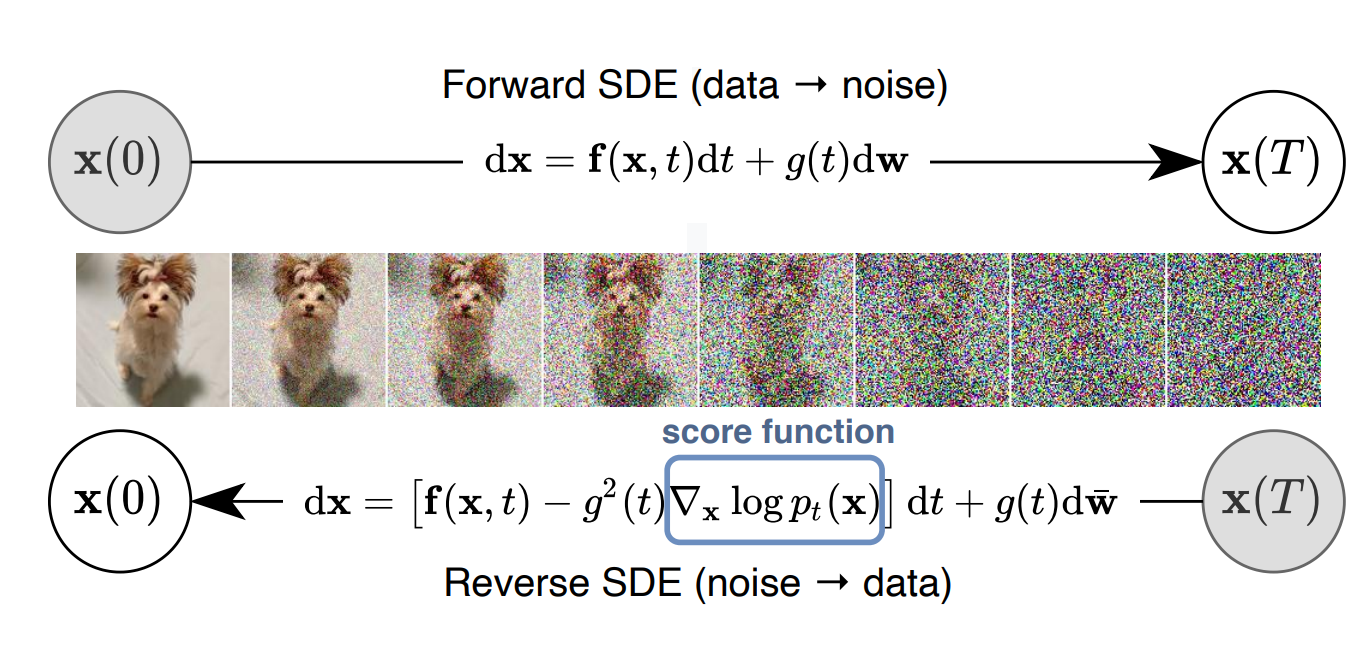
\includegraphics[width=0.7\textwidth]{SDE.png}
    \centering 
  \end{figure}
  \item \textbf{Probability flow ODE} introduced by \textit{Song et. el (2020)} has the same marginals as the reverse SDE 
  \begin{align}
    \dd \mathbf{x}_t = \left[\mathbf{f}(\mathbf{x}_t, t) - \frac{1}{2}g(t)^2 \nabla_\mathbf{x} \log q_t(\mathbf{x}_t)\right] \dd t 
  \end{align}
\end{itemize}
\end{frame}

\begin{frame}{Simplified derivation}
\begin{itemize}
  \item Starting with a forward SDE
  \begin{align}
    \dd \mathbf{x}_t = \mathbf{f}(\mathbf{x}_t, t) \dd t + g(t)\dd \mathbf{w}_t, 
  \end{align}
  we can write \underline{Kolmogorov Forward Equation} for its marginal densities
  \begin{align}
    \frac{\partial q_t(\mathbf{x})}{\partial t} = -\nabla_{\mathbf{x}} \cdot \left[\mathbf{f}(\mathbf{x}, t)q_t(\mathbf{x}) - \frac{1}{2}g^2(t) \nabla_{\mathbf{x}} q_t(\mathbf{x})\right]
  \end{align}
  \item Using $\nabla_{\mathbf{x}} \log q_t(\mathbf{x}) = \frac{\nabla_{\mathbf{x}} q_t(\mathbf{x})}{q_t(\mathbf{x})}$ we can rewrite 
  \begin{align}
    \frac{\partial q_t(\mathbf{x})}{\partial t} = -\nabla_{\mathbf{x}} \cdot \left[(\mathbf{f}(\mathbf{x}, t) - \frac{1}{2}g^2(t) \nabla_{\mathbf{x}} \log q_t(\mathbf{x})) q_t(\mathbf{x}) \right]
  \end{align}
\end{itemize}
\end{frame}

\subsubsection{Training of and sampling from score SDEs}
\begin{frame}{Training of and sampling from score SDEs}
\begin{itemize}
  \item Once we know $q_t(\mathbf{x})$, sampling is straightforward either from the SDE with annealed Langevin dynamics or from the probability flow ODE with some numerical ODE solver
  \item We don't know $q_t(\mathbf{x})$ and obtaining it directly from KFE isn't really feasible, hence score matching again for $t \sim \mathcal{U}[0, T], \mathbf{x}_0 \sim q(\mathbf{x}_0), \mathbf{x}_t \sim q(\mathbf{x}_t \mid \mathbf{x}_0)$
  \begin{align}
    \mathbb{E}_{t, \mathbf{x}_0, \mathbf{x}_t}\left[\lambda(t)\norm{\mathbf{s}_\theta(\mathbf{x}, t) - \nabla_{\mathbf{x}_t} \log q_{0t}(\mathbf{x}_t \mid \mathbf{x}_0)}^2\right]
  \end{align}
\end{itemize}
\end{frame}

\section{Directions of improvement (Chapters 3-4)}
\begin{frame}{Directions of improvement}
Subsequent research on diffusion models focuses on improving these classical approaches
(DDPMs, SGMs, and Score SDEs) from three major directions:
\begin{enumerate}
  \item faster and more efficient sampling;
  \item more accurate likelihood and density estimation;
  \item handling data with special structures (such
  as permutation invariance, manifold structures, and discrete data).
\end{enumerate}
\end{frame}

\subsection{Efficient sampling}
\begin{frame}{Efficient sampling}
\begin{itemize}
  \item The main goal is in improving either SDE or ODE solvers, decreasing the number of discretized time steps, while minimizing the error.
  \item \textbf{Learning-free} sampling is a paradigm of using handcrafted steps, while \textbf{learning-based} sampling is based on optimizing certain learning objectives.
\end{itemize}
\end{frame}

\subsubsection{Learning-free sampling}
\begin{frame}{Learning-free sampling}
Some SDE improvements
\begin{itemize}
  \item \textbf{Predictor-corrector for SDE}: coarse SDE solver (predictor) and iterative MCMC procedure to nudge it to the correct marginal (corrector) 
  \item \textbf{Adaptive step size}: from \textit{Jolicoeur-Martineau et al. (2021)} there is an SDE solver with adaptive step sizes for faster generation, based on comparing a high-order and a low-order SDE solvers
\end{itemize}
Some ODE improvements
\begin{itemize}
  \item \textbf{Diffusion Exponential Integrator Sampler} utilizes semi-linear structure of probability flow ODE to get an edge over  the general-purpose methods, for DDPM 
  \begin{align}
    \dd \mathbf{x}_t = \left[-\frac{1}{2}\beta_t \mathbf{x}_t - \frac{1}{2}\beta_t \nabla_{\mathbf{x}}\log q_t (\mathbf{x}_t)\right] \dd t
  \end{align}
\end{itemize}
\end{frame}

\subsubsection{Learning-based sampling}
\begin{frame}{Learning-based sampling}
\begin{itemize}
  \item \textbf{Optimized discretization}: given a pre-trained model, we are looking for the best $K$ time-steps, this optimization becomes feasible with use of dynamic programming 
  \item \textbf{Truncated diffusion}: truncating forward and reverse diffusion processes, starting denoising earlier and generating initial samples with some pre-trained generative model 
\end{itemize}
\end{frame}

\subsection{Improved likelihood (introduction)}
\begin{frame}{Improved likelihood (introduction)}
\begin{itemize}
  \item VLB of the log-likelihood is not a tight bound in many cases, so optimizing it leads to suboptimal resutls
  \item We want to achieve likelihood maximization and there are three methods 
  \begin{enumerate}
    \item noise schedule optimization;
    \item \textbf{reverse variance learning}; 
    \item exact log-likelihood evaluation.
  \end{enumerate}
\end{itemize}
\end{frame}

\subsubsection{Reverse variance learning}
\begin{frame}{Reverse variance learning}
\begin{itemize}
  \item Even though we introduced $\Sigma_\theta (\mathbf{x}_t, t)$ in DDPM formulation, in practice people used $\beta \mathbf{I}$ in place of it (no learning)
  \item The idea of the \textbf{reverse variance learning} is to write a representation which will allow to efficiently learn the reverse variance 
  \begin{align}
    \Sigma_\theta = \exp(\theta \cdot \log \beta_t + (1-\theta)\cdot \log \tilde{\beta}_t), \quad \tilde{\beta}_t = \frac{1-\overline{\alpha}_{t-1}}{1-\overline{\alpha}_{t}}
  \end{align}
  \item Jointly train $\beta_t$ and $\theta$ to maximize VLB.
  \item In \textit{Analytic-DPM} they found an optimal reverse variance if one knows the score functions. 
\end{itemize}
\end{frame}


\end{document}